\newpage
\section{Aufbau}
\label{sec:Durchführung}

\begin{floatingfigure}{0.55\textwidth}
  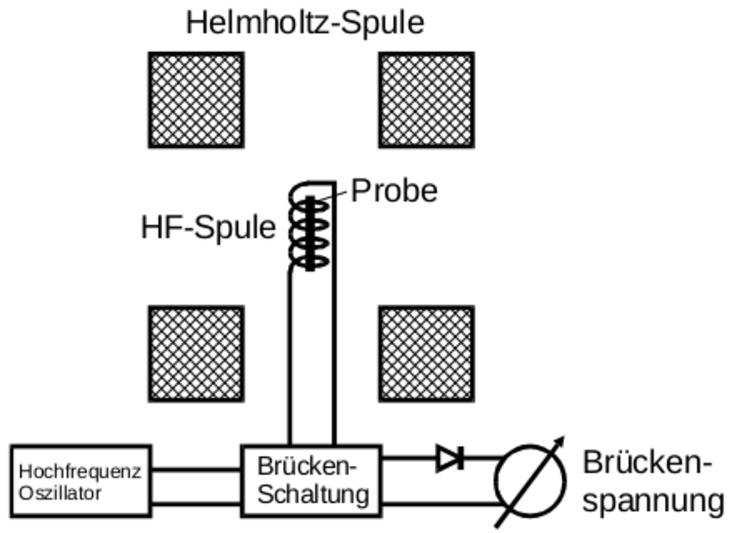
\includegraphics[width=0.55\textwidth]{picture/schematischerAufbau.pdf}
  \caption{Schematischer Aufbau einer Elektronenspin-Resonanz Apparatur. \cite{V28}}
  \label{fig:schematischerAufbau}
\end{floatingfigure}

Der schematische Aufbau einer ESR-Apparatur ist in Abbildung \eqref{fig:schematischerAufbau} zu sehen. In dem homogenen Magnetfeld der Helmholtzspulen befindet sich die zu untersuchende Probe. Um die Probe ist eine Hochfrequenz-Spule gewickelt, diese Spule wird über eine Brückenschaltung von einem Hochfrequenz-Generator gespeist (vgl. \cite[109]{V28}). Für diesen Aufbau übernimmt das hochfrequente Magnetfeld die Aufgabe der Photonen und induziert den Übergang. Dadurch ändert sich die Magnetisierung der Probe und in folge dessen auch der komplexe Widerstand der Hochfrequenz-Spule. An der vorher abgeglichen Brückenschaltung tritt nun eine Brückenspannung auf, welche mit einem empfindlichen Messinstrument nachgewiesen werden kann. Die Brückenschaltung ist in Abbildung \eqref{fig:realerAufbau} zu sehen. Da die dabei auftretenden Spannungen sehr klein sind, müssen diese verstärkt werden. Für diesen Zweck wird ein Überlagerungsempfänger verwendet. Der Aufbau ist in Abbildung \eqref{fig:Überlagerungsempfänger} dargestellt. Zu Beginn verstärkt der Vorverstärker die Signalfrequenz $\nu_\text{e}$ leicht. Dieses Signal wir in einer Mischstufe mit einem Signal $\nu_\text{Osz}$ überlagert, wodurch Schwebungserscheinungen mit der Frequenz
\begin{align}
  \nu_\text{ZF} = \nu_\text{e} - \nu_\text{Osz}
\end{align}
auftreten. Der Selektiv-Verstärker verstärkt nun das Signal $\nu_\text{Osz}$ stark und unterdrückt Störfrequenzen. Je weiter die Störfrequenzen von der Signalfrequenz entfernt sind, desto besser werden die Störfrequenzen unterdrückt. Zuletzt wird die hochfrequente Wechselspannung durch eine Demodulatorstufe gleichgerichtet und geglättet.

\begin{figure}
  \centering
  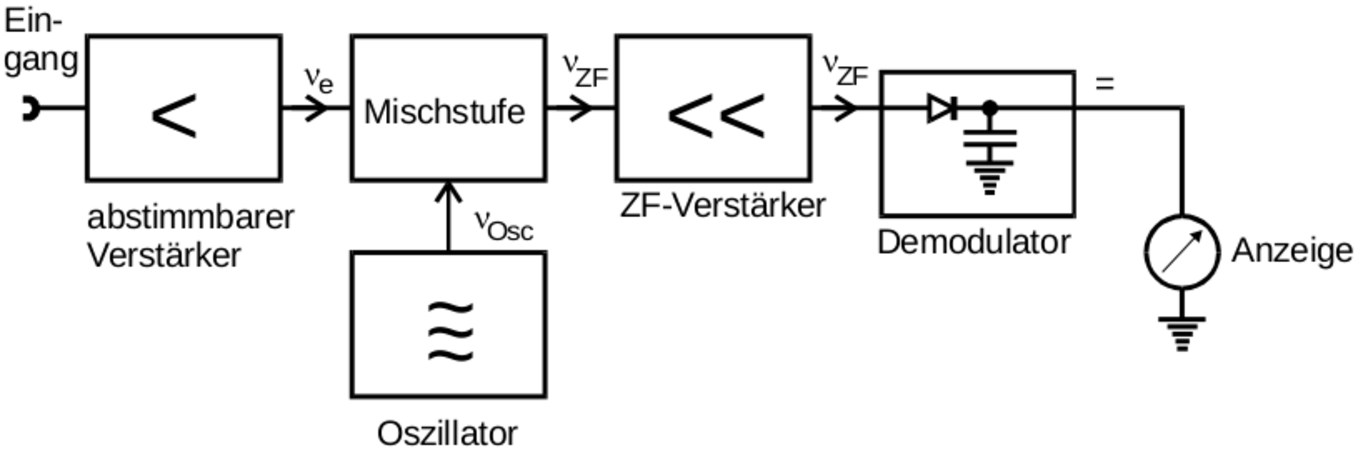
\includegraphics[width=\textwidth]{picture/Überlagerungsempfänger.pdf}
  \caption{Blockschaltbild eines Überlagerungsempfängers. \cite{V28}}
  \label{fig:Überlagerungsempfänger}
\end{figure}

\newpage
\begin{figure}
  \centering
  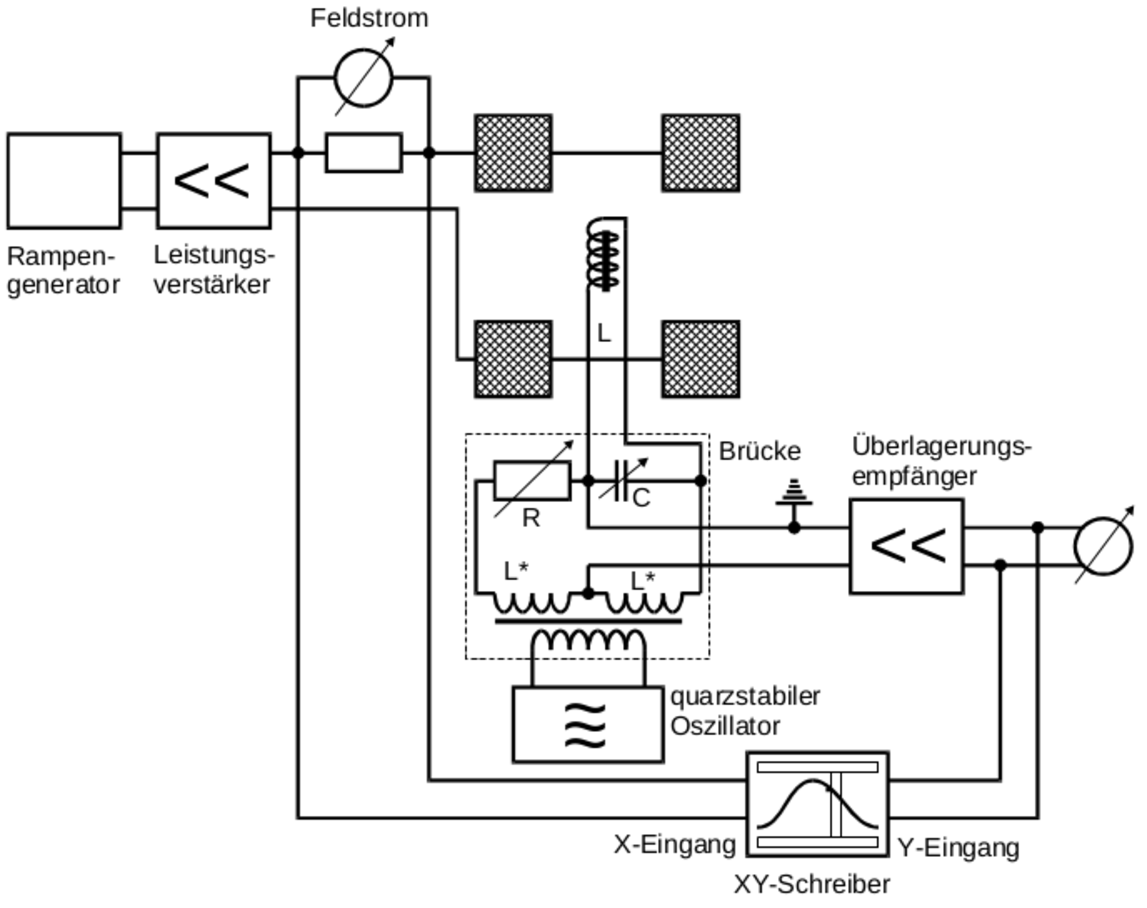
\includegraphics[width=\linewidth]{picture/realerAufbau.pdf}
  \caption{Detaillierter Versuchsaufbau für die Elektronenspin-Resonanz. \cite{V28}}
  \label{fig:realerAufbau}
\end{figure}



\section{Durchführung}
Da mit Magnetfeldern im Bereich von mT gearbeitet wird, muss das Erdmagnetfeld beachtet werden. Deshalb werden alle Messungen sowohl parallel, als auch antiparallel zum Erdmagnetfeld durchgeführt. \\
Im nächsten Schritt wird die Brücke und der Empfänger auf die gewünschte Frequenz abgestimmt. Dazu wird die  Oszillator-Frequenz $\nu_\text{Osz}$ so eingestellt, dass
\begin{align}
  \nu_\text{Osz} + \nu_\text{ZF} = \nu_\text{e}
\end{align}
gilt. Die Verstärker werden auf die maximale Verstärkung eingestellt. Dann wird versucht die Brückenspannung, mit Hilfe von zwei Kapazitäten $C_\text{grob}$ und $C_\text{fein}$ und einem Widerstand $R$ zu minimieren. Danach wird der Feldstrom an den $x$-Eingang des XY-Schreibers angeschlossen und die Brückenspannung an den $y$-Eingang. Dann wird über einen Rampengenerator ein gleichmäßig steigender Feldstrom auf die Helmholzspule gegeben. \\
Zu letzt wird die $x$-Achse des XY-Schreibers kallibriert, in dem mehrere Punkte mit bekanntem Strom auf dem Papier gesetzt werden. Dadurch kann der Strom pro cm bestimmt werden. \\
Der gesamte Vorgang wird für fünf verschiedene Frequenzen wiederholt.
